\subsection{Swing-up}
\label{sec:Results_swingup}
Finally, a comparison of two different strategies for swing-up is presented in this section. Both the swing-up strategies are model-based. The first strategy is an energy-based swing-up law adopted from Fantoni et al.~\cite{Fantoni}. Figure \ref{fig:swing_up} shows the evolution of the arm and pendulum angles from down-down configuration at $\phi_1 = \phi_2 = 180^\circ$ to up-up configuration with $\phi_1 = \phi_2 = 0^\circ.$ The approach presented in \cite{Fantoni} ensures that the arm swings up and brings the pendulum into a homoclinic orbit where a stabilizing controller takes over from the energy-based controller and thereafter performs a regulation task to the up-up configuration. The parameters were tuned by a GA which resulted in $k_E = 4.55 $, $k_P = 0.4$, and $k_D = 0.8$. Similarly, Figure~\ref{fig:swing_up_qLMPC} shows the evolution of arm and pendulum angles for a swing-up approach based on the previously introduced qLPV-MPC approach. Here, only one controller is sufficient for both swinging up the pendulum and stabilizing it about the up-up configuration. The swing-up parameters were GA tuned; the parameters are $\mathbf{Q} = \textup{diag}(2623,~746.36,~46.65,~0.51))$ and $\textup{R} = 61.4$ and $\mathbf{Q}_N = 427.25\mathbf{Q}$. Furthermore, Figure \ref{fig:Etilda} shows the change in the system's total energy. The energy-based swing-up law performs significantly better than the qLMPC swing-up law. However, the latter has the advantage that it is just a single controller, unlike the former, which requires an additional stabilizing controller. 
% 
\begin{figure}[H]
    \centering
    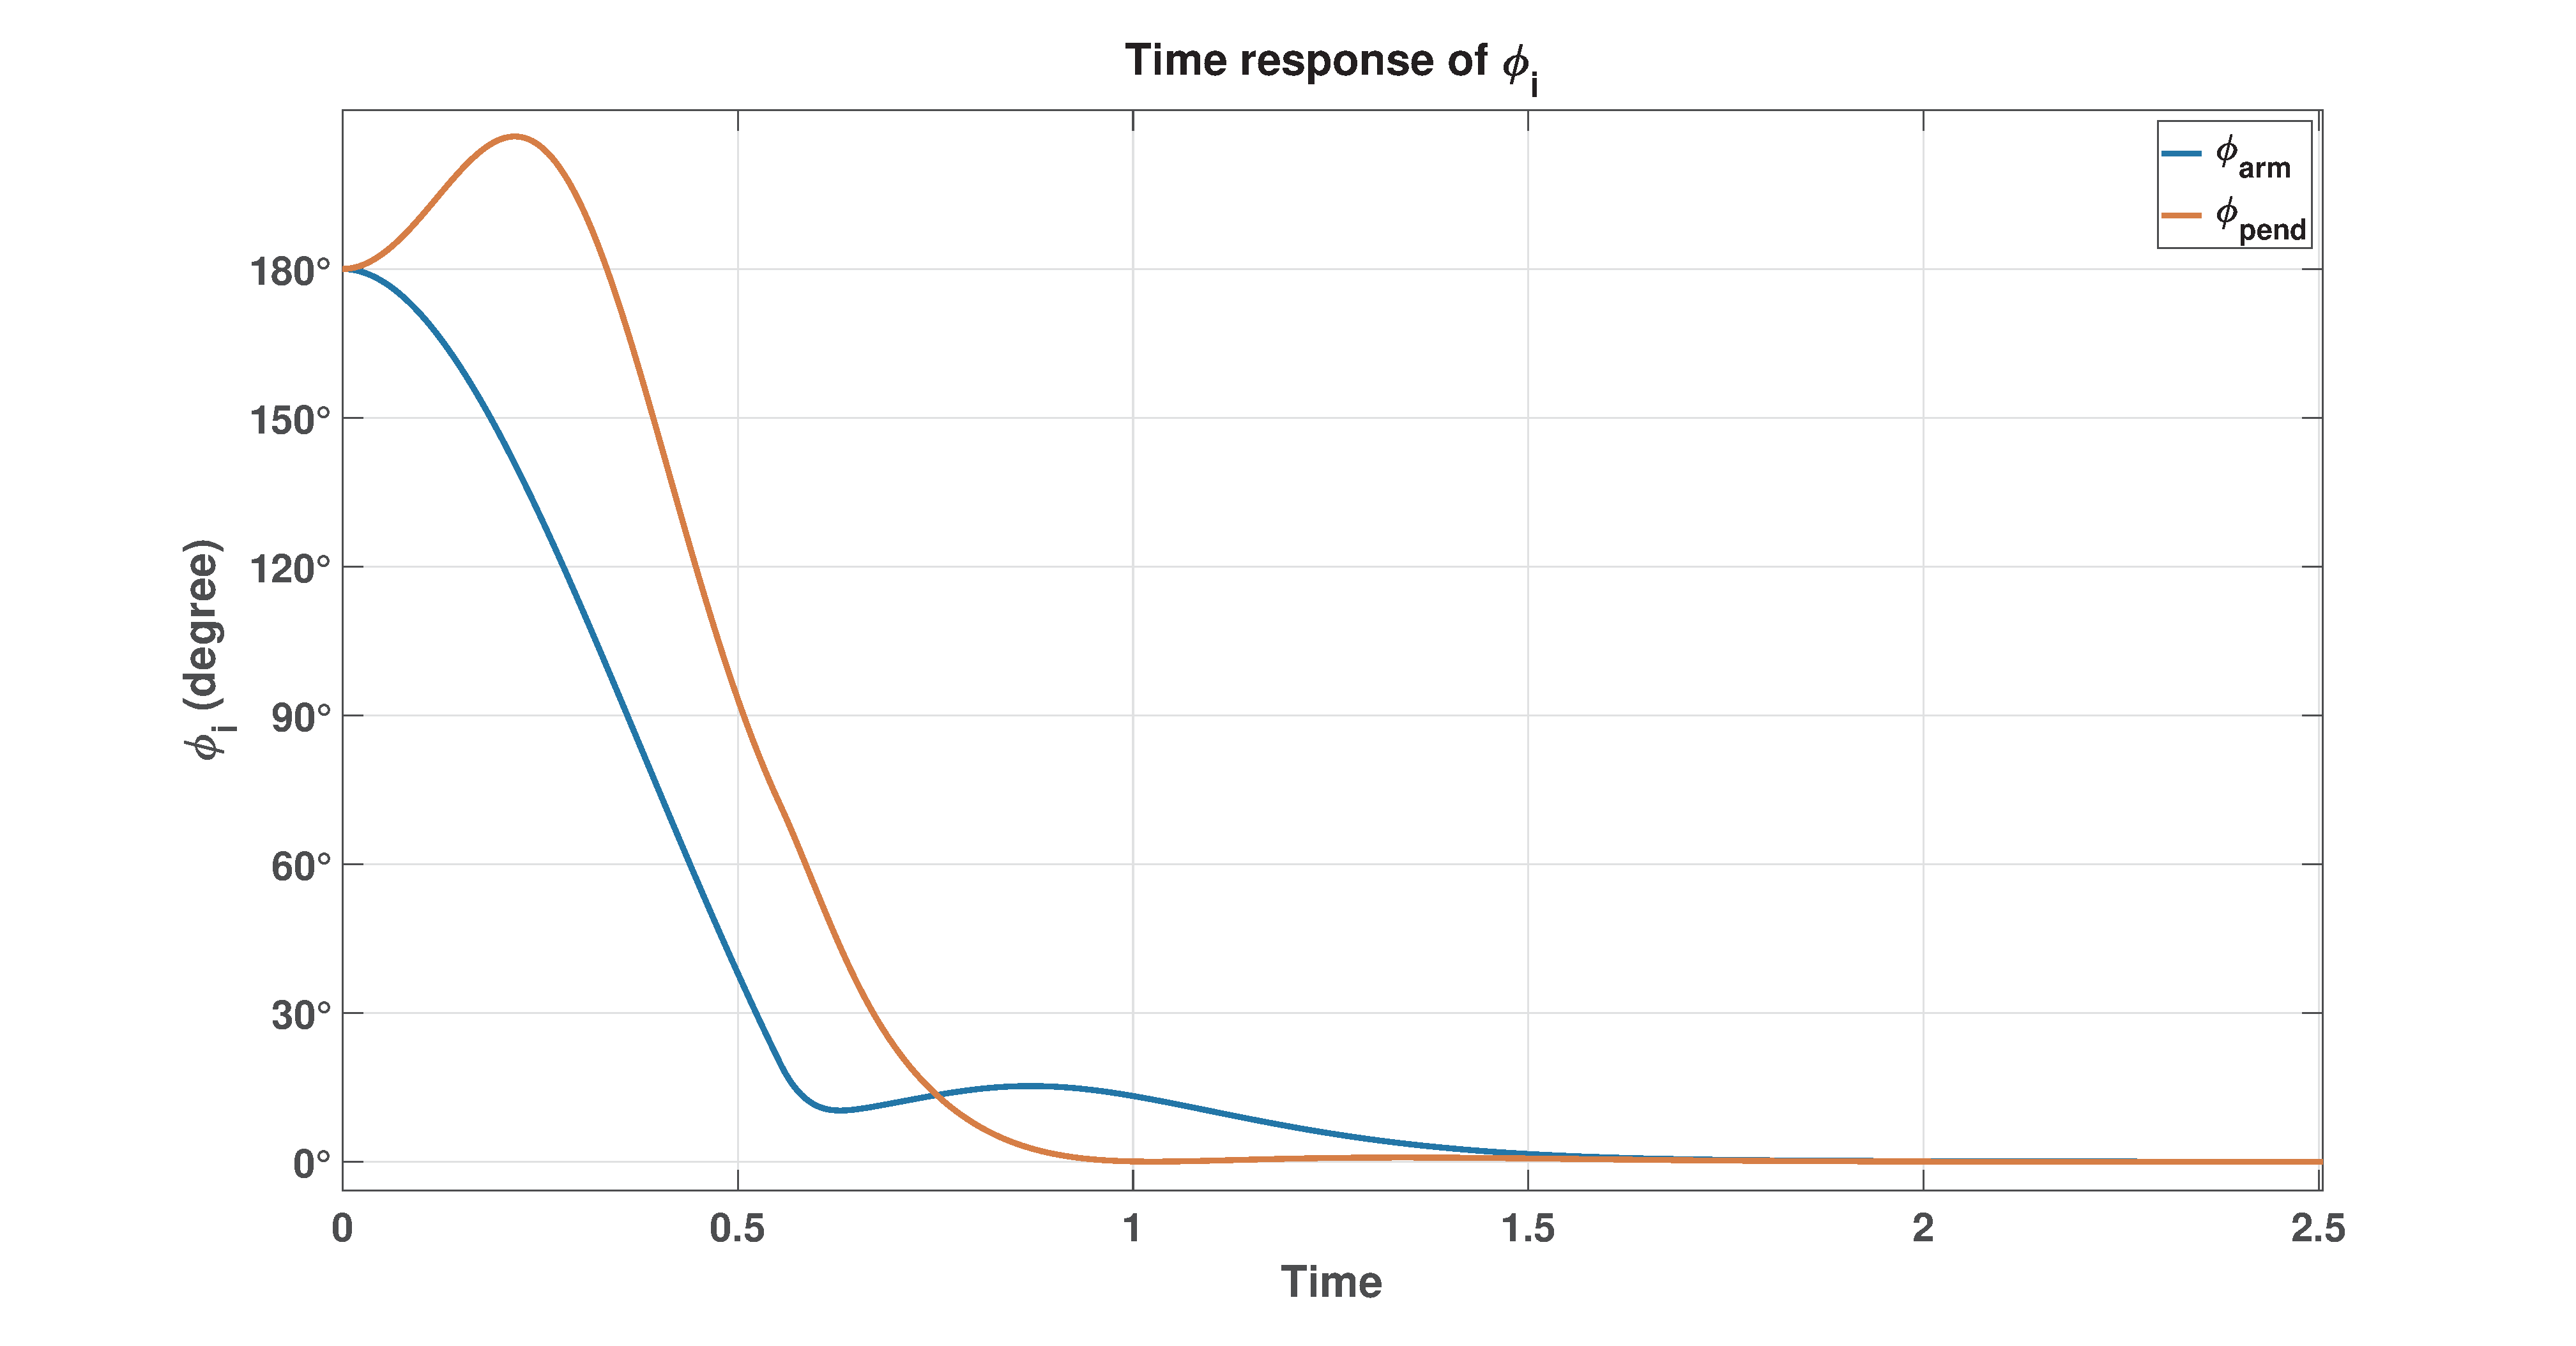
\includegraphics[width=0.84\textwidth]{figures/Swing_up}
    \caption{Swing-up performed by energy-based controller and a stabilizing LQR.}
    \label{fig:swing_up}
% \end{figure}
\vspace{0.004em}
% \begin{figure}[ht]
    \centering
    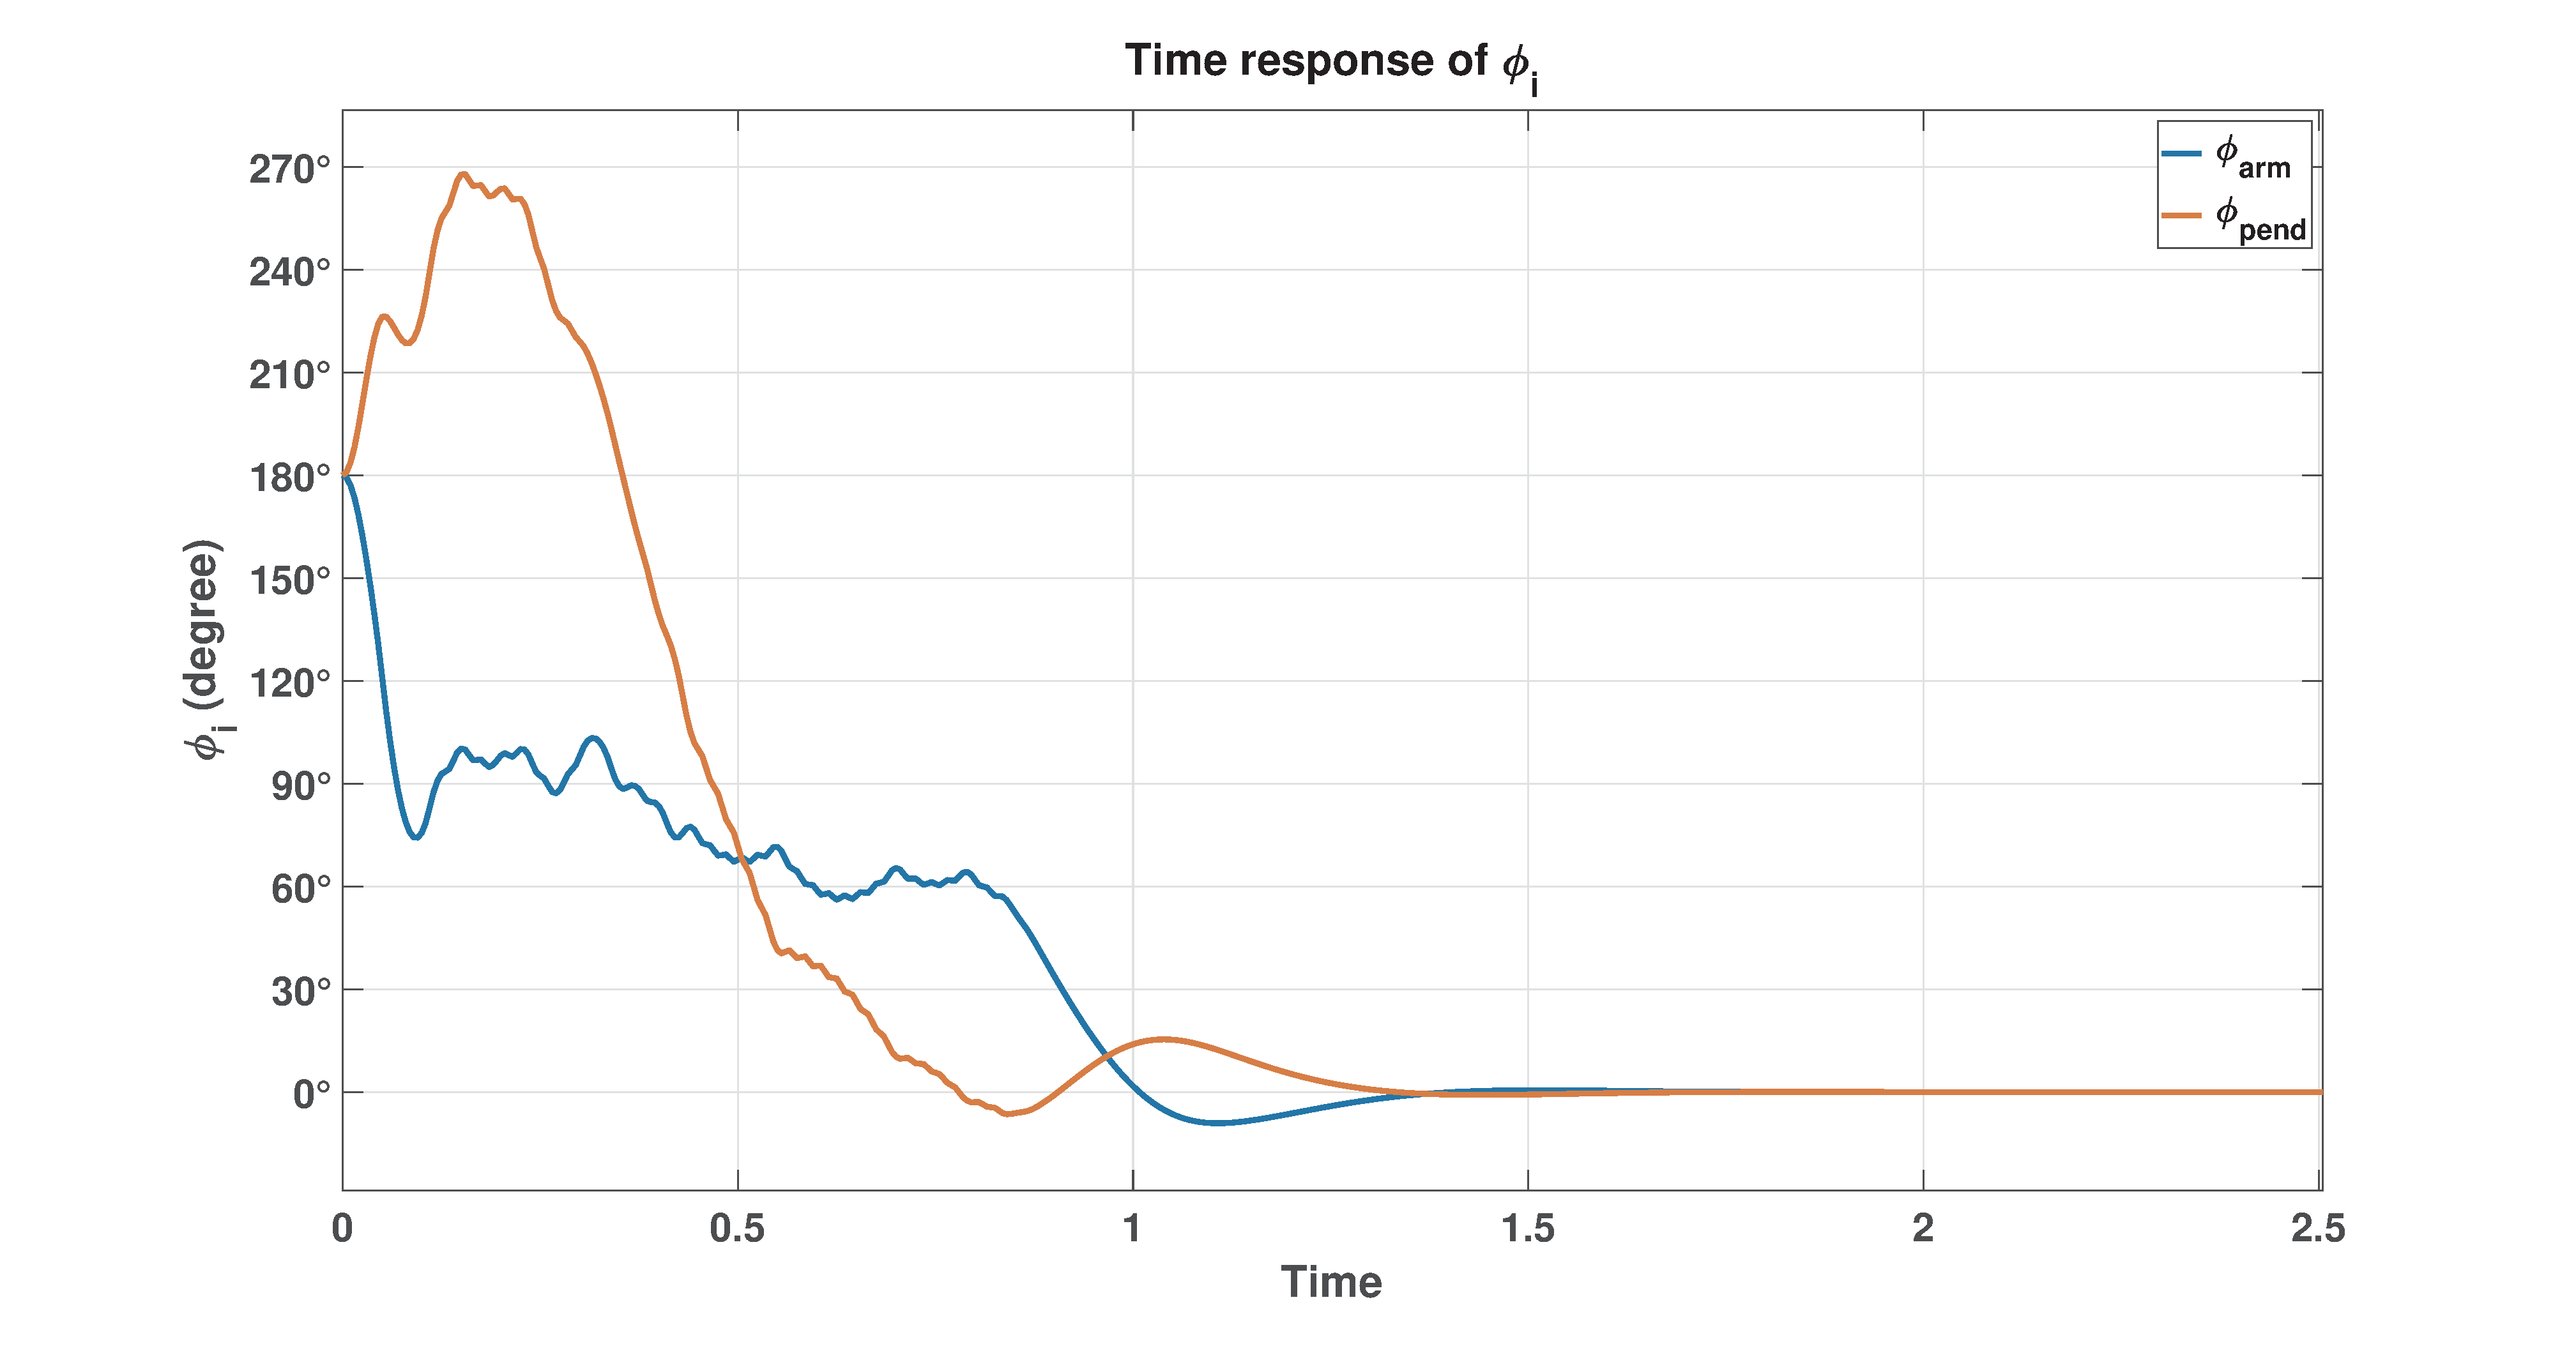
\includegraphics[width=0.84\textwidth]{figures/qLMPC_swingup}
    \caption{Swing-up performed by qLPV-MPC controller}
    \label{fig:swing_up_qLMPC}
% \end{figure}%
\vspace{0.004em}
% \begin{figure}[ht]
    \centering
    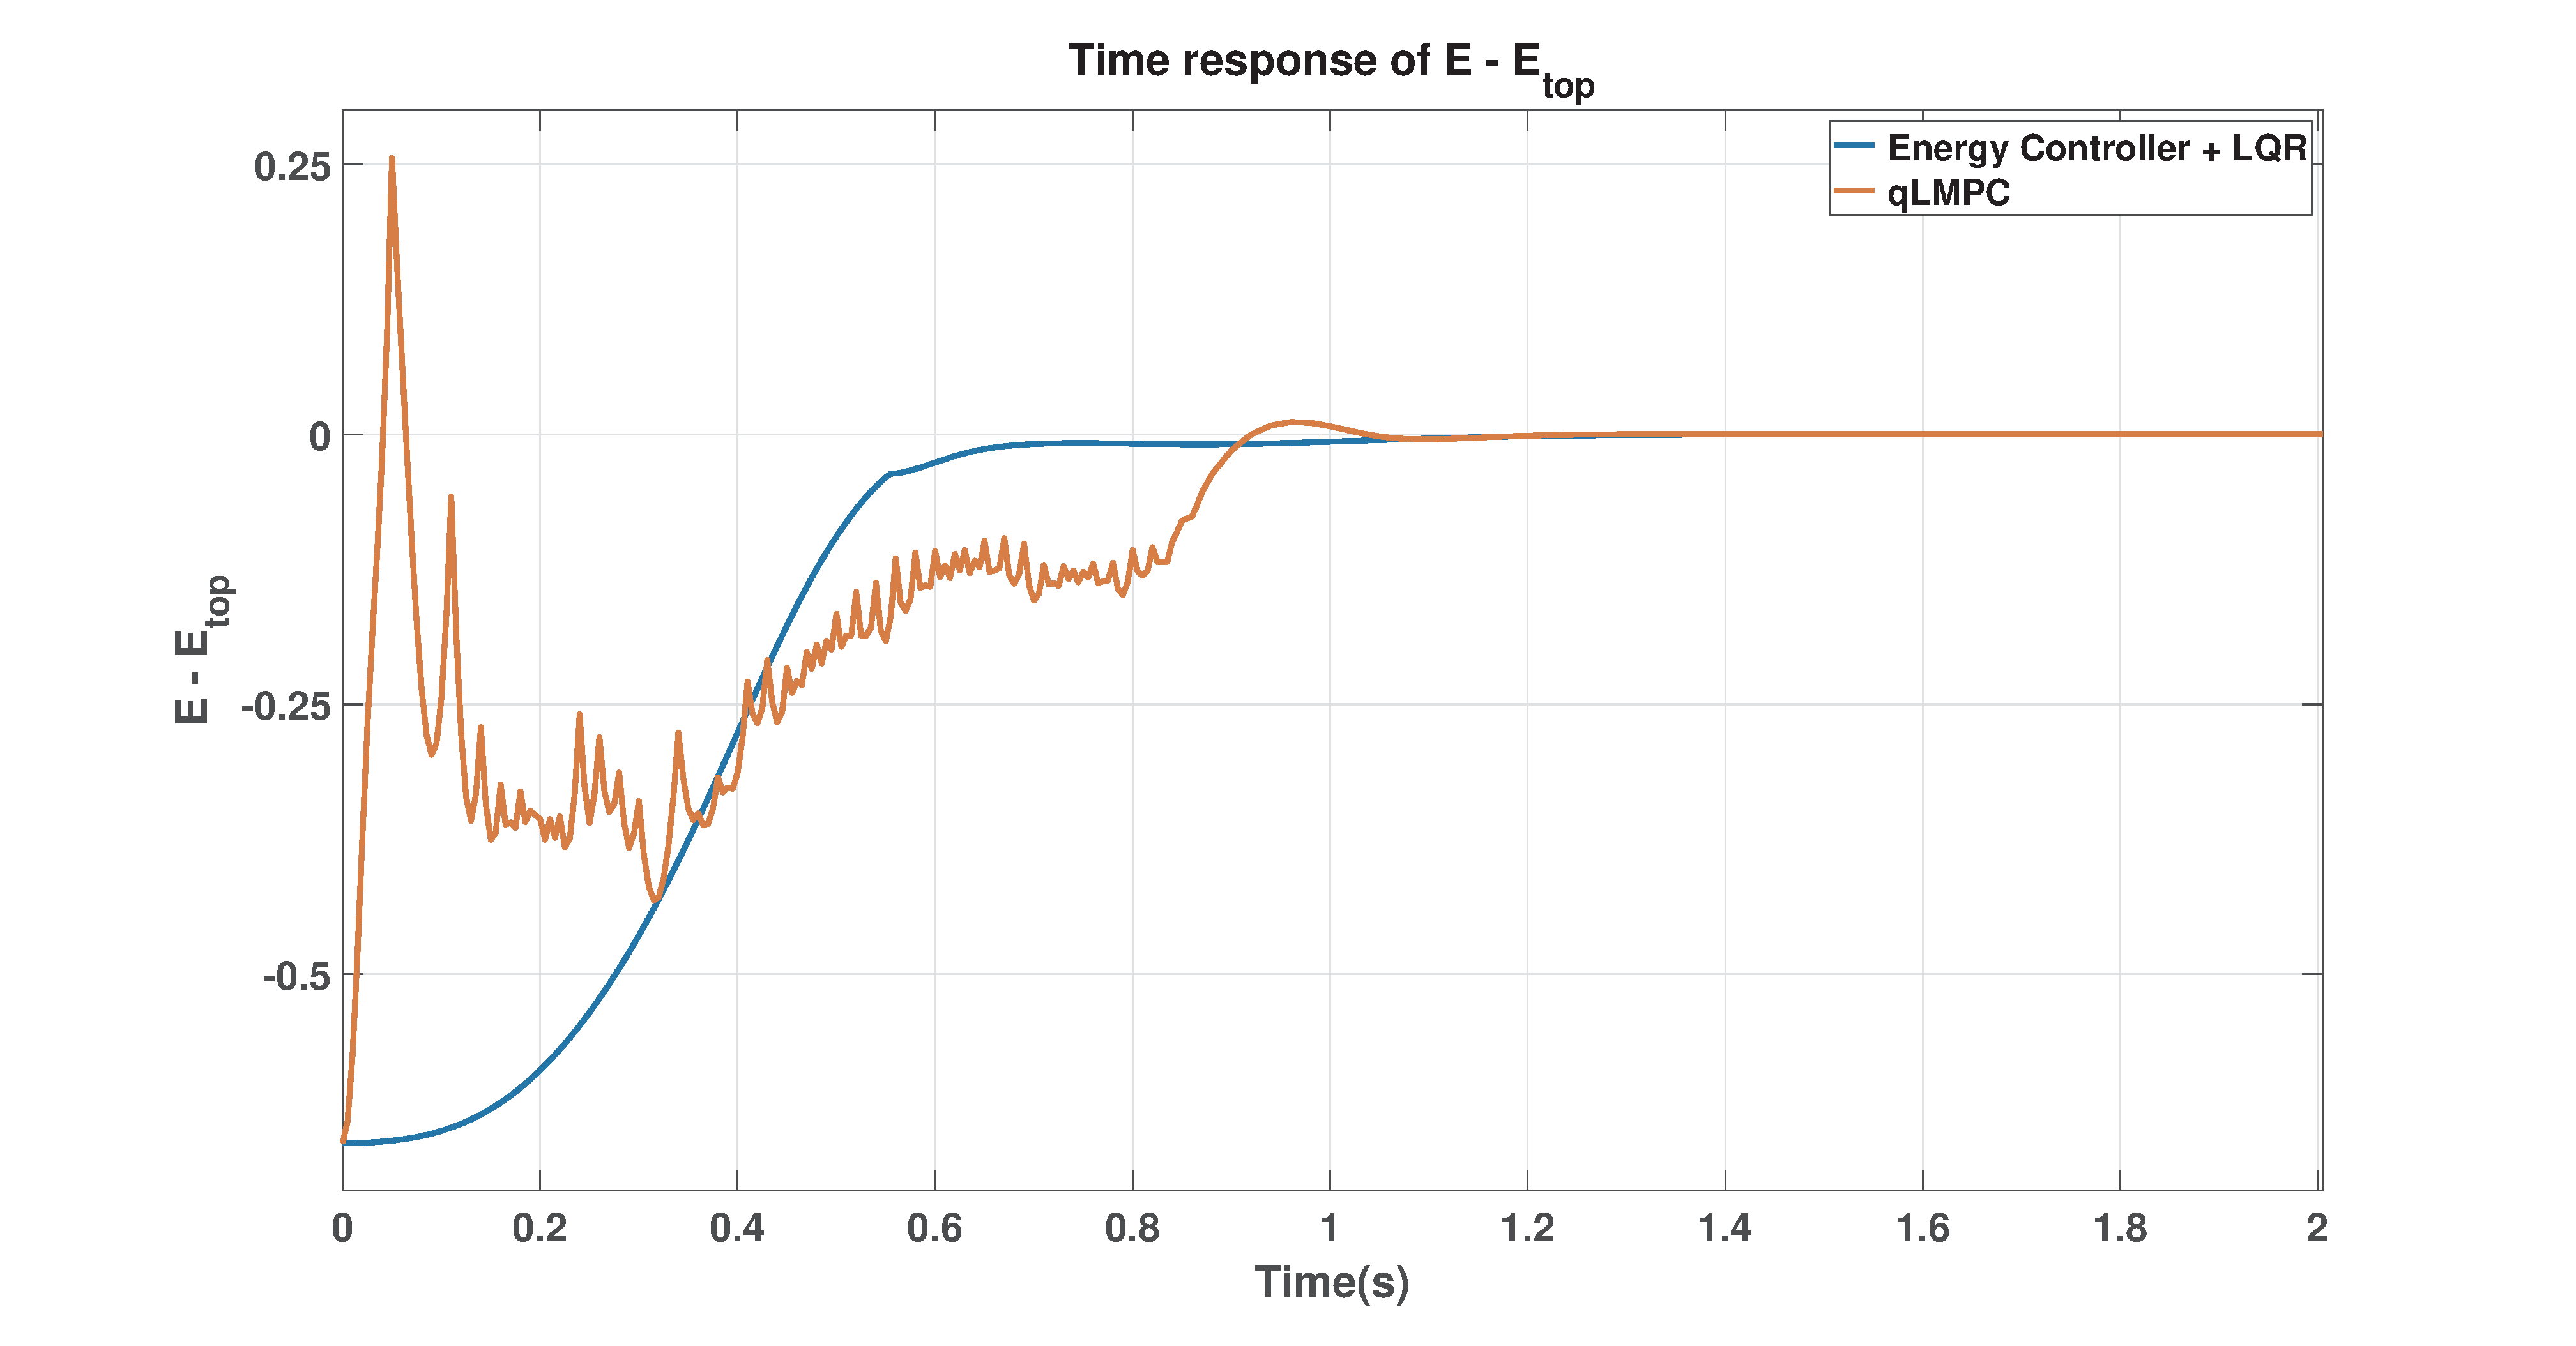
\includegraphics[width=0.84\textwidth]{figures/Etilda_comb}
    \caption{Time response of $\tilde{E}$.}
    \label{fig:Etilda}
\end{figure}
    % ~
    % \begin{subfigure}[t]{0.485\textwidth}
    % \centering
    % 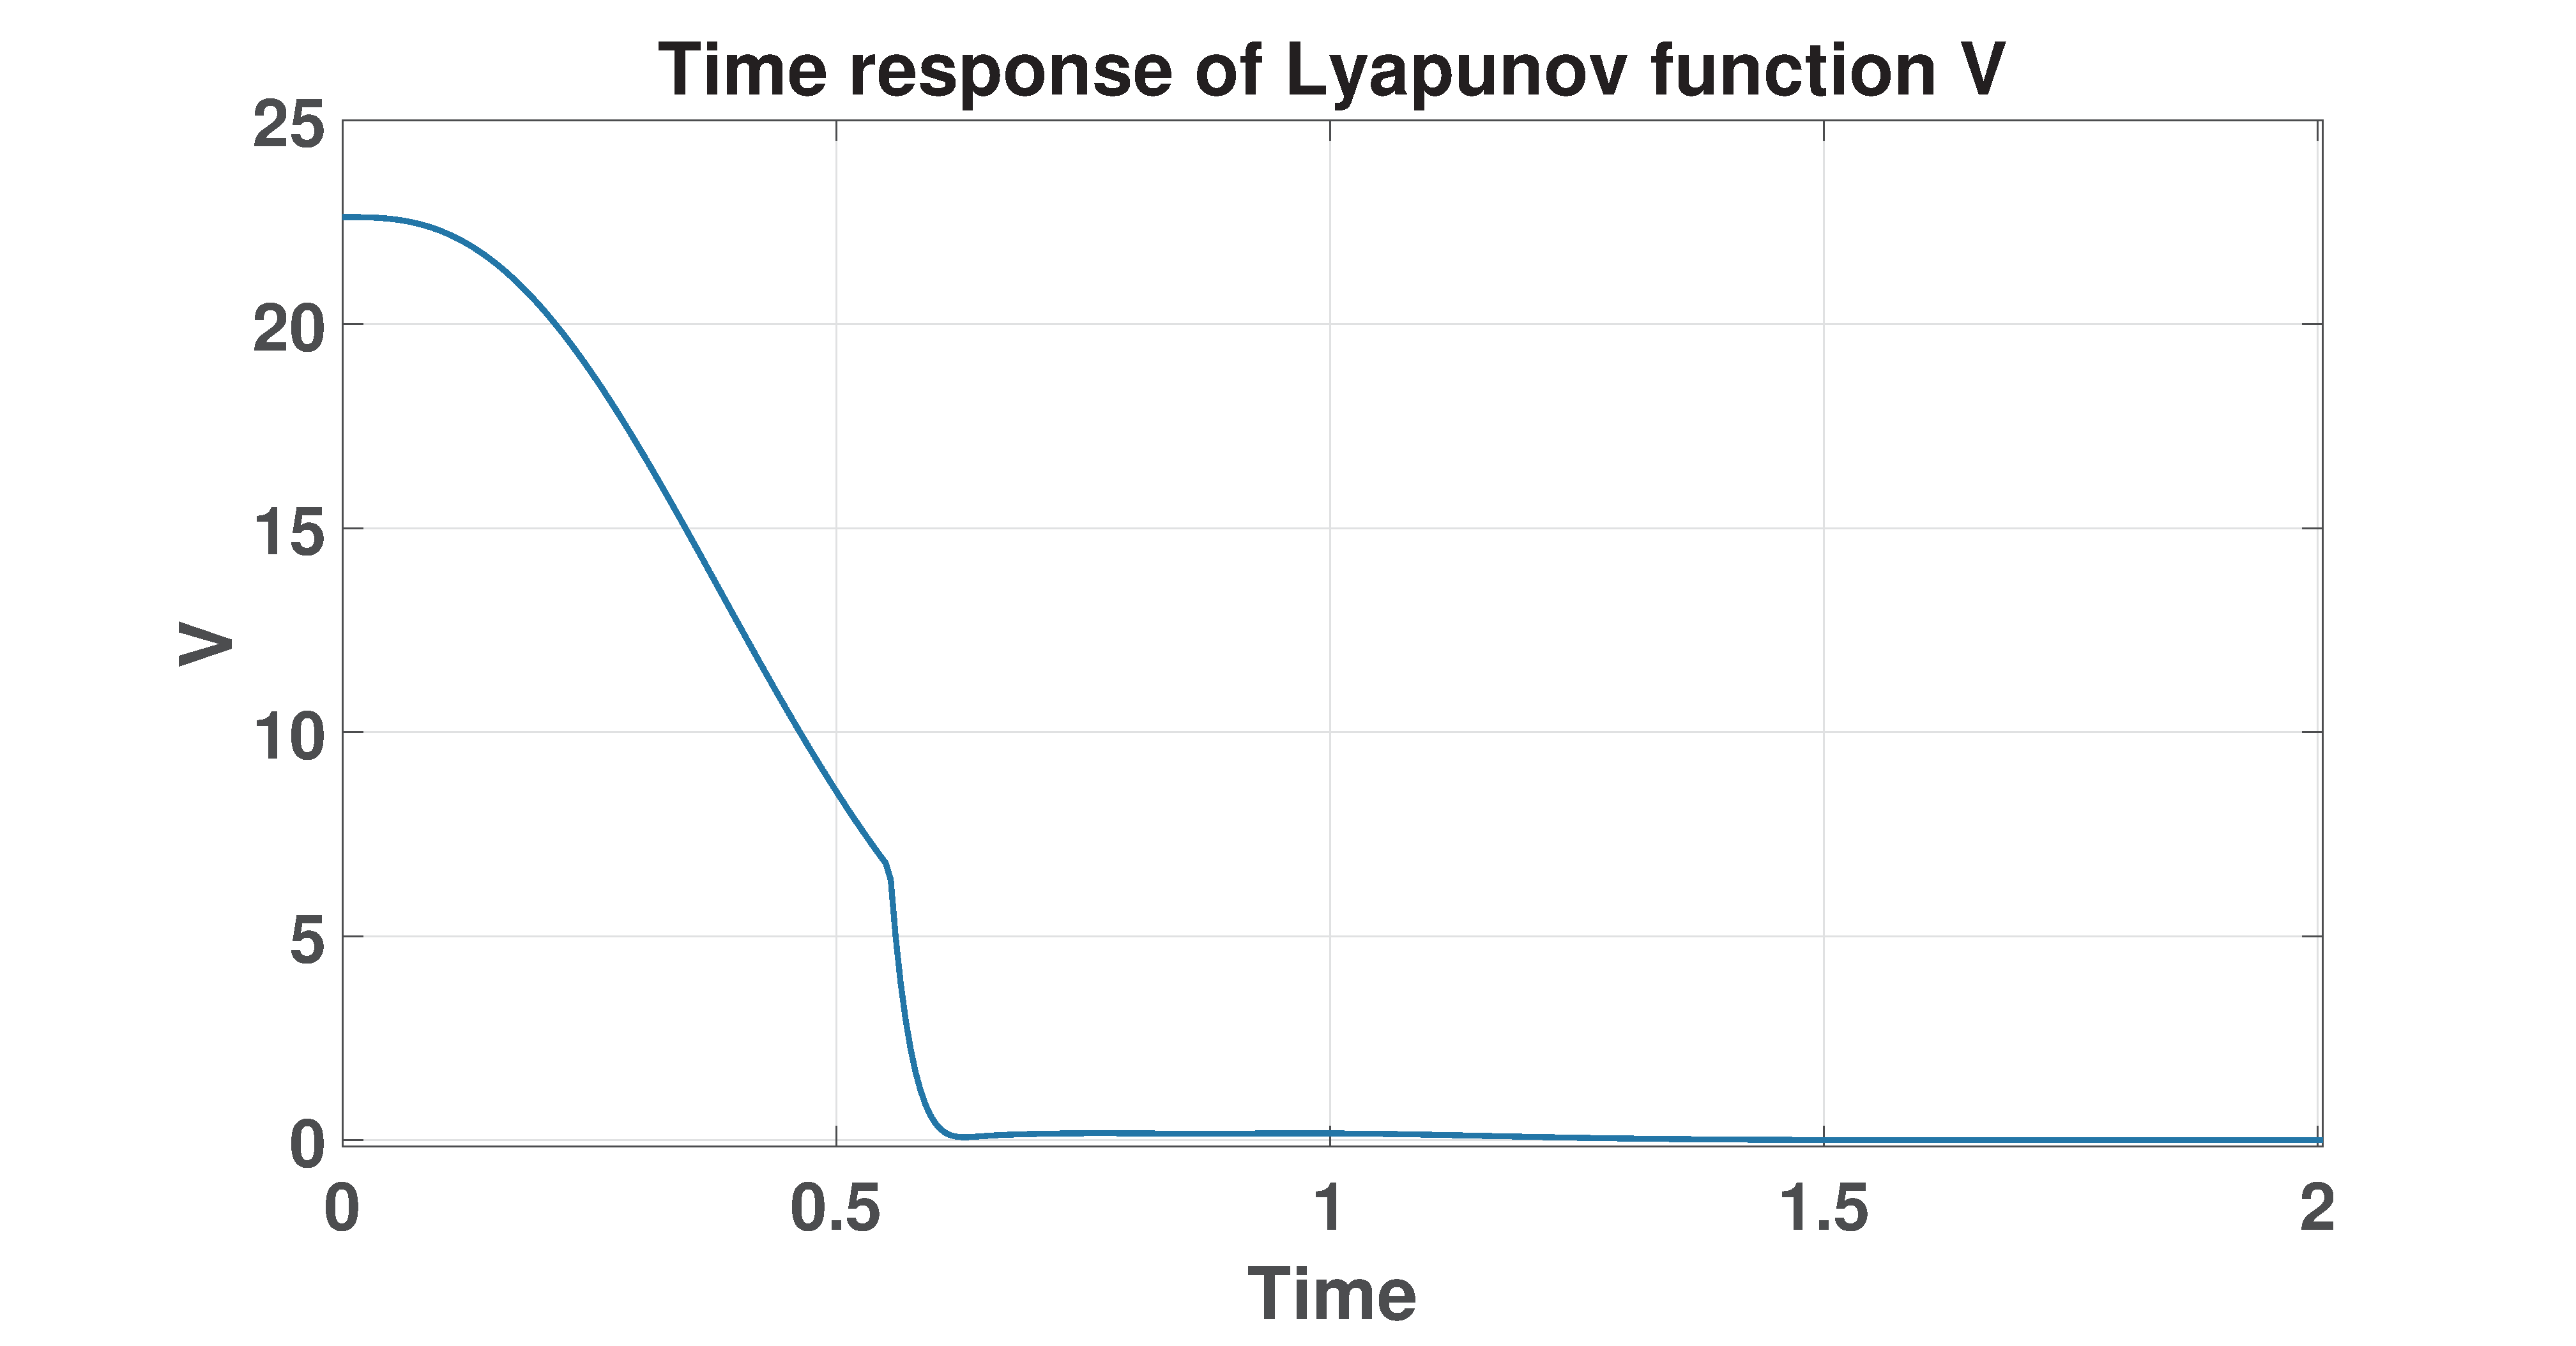
\includegraphics[width=\textwidth]{figures/Lyapunov}
    % \caption{Time response of Lyapunov function $V$.}
    % \label{fig:Lyapunov}
    % \end{subfigure}
    % \caption{Time responses}
% \end{figure}